\documentclass[border=5pt]{standalone}
\usepackage{tikz}
\usetikzlibrary{decorations.pathreplacing}
\usepackage{xcolor}

\definecolor{SeventyBlack}{HTML}{5C5C5C}
\definecolor{Atlantic}{HTML}{466A9F}

\tikzset{every node/.append style={rounded corners=0pt}}

\begin{document}
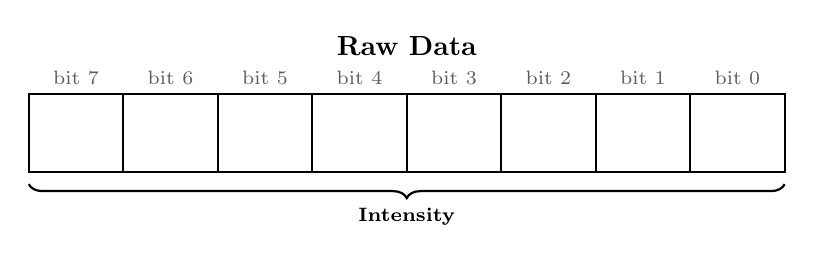
\begin{tikzpicture}

\node[font=\normalsize\bfseries] at (4.8, 4.6) {Raw Data};

\foreach \i/\v in {0/7, 1/6, 2/5, 3/4, 4/3, 5/2, 6/1, 7/0} {
    \node[font=\scriptsize, color=SeventyBlack] at (0.6 + \i*1.2, 4.2) {bit \v};
}

\foreach \i in {0,...,7} {
    \draw[thick] (0 + \i*1.2, 3.0) rectangle (1.2 + \i*1.2, 4.0);
}

\draw[decorate, decoration={brace, amplitude=5pt, mirror}, thick]
    (0, 2.85) -- (9.6, 2.85) node[midway, below=5pt, font=\scriptsize\bfseries] {Intensity};

\end{tikzpicture}
\end{document}
